\section{实验设置及结果}

为了使优化器的通用性和可扩展性,实验基于PyTorch的Optimizer类进行优化器实现,并分别实现了随机搜索优化器,梯度下降优化器,次梯度下降优化器,共轭方向优化器,共轭梯度优化器,变尺度法优化器(BFGS),随机梯度下降优化器,Newton优化器,阻尼Newton优化器,ADMM优化器和Krylov子空间优化器,并使用Rosenbrock Banana函数作为优化器测试函数,即
\begin{equation*}
    f(x_1, x_2)=(a-x_1)^2-b(x_2-x_1^2)^2 \text{,}
\end{equation*}
其中$a=1$,$b=-100$。
实验结果如\cref{table:result}所示,各优化器的最优值收敛曲线和最优点收敛路径如\cref{figure:random search}至\cref{figure:krylov}所示。

\begin{table}[ht]
    \centering
    \caption{实验结果}
    \label{table:result}
    \begin{tabular}{cccc}
        \toprule
        \textbf{优化器} & \textbf{最优点} & \textbf{最优值} & \textbf{迭代轮次} \\
        \midrule
        Random Search & $(1.00, 1.00)$ & 0.00 & 1326 \\
        Gradient Descent & $(0.99, 1.00)$ & 0.00 & 10808 \\
        Subgradient Descent & $(0.99, 1.00)$ & 0.00 & 10808 \\
        Conjugate Direction & $(1.00, 1.00)$ & 0.00 & 23366 \\
        Conjugate Gradient & $(1.00, 1.00)$ & 0.00 & 500 \\
        BFGS & $(1.00, 1.00)$ & 0.00 & 21983 \\
        SGD & $(1.00, 1.00)$ & 0.00 & 6350 \\
        Newton & $(1.00, 1.00)$ & 0.00 & 7 \\
        Damped Newton & $(1.00, 1.00)$ & 0.00 & 2970 \\
        ADMM & $(1.00, 1.00)$ & 0.00 & 22184 \\
        Krylov & $(1.00, 1.00)$ & 0.00 & 6385 \\
        \bottomrule
    \end{tabular}
\end{table}

\begin{figure}[!ht]
    \centering
    \begin{subfigure}{0.4\textwidth}
        \centering
        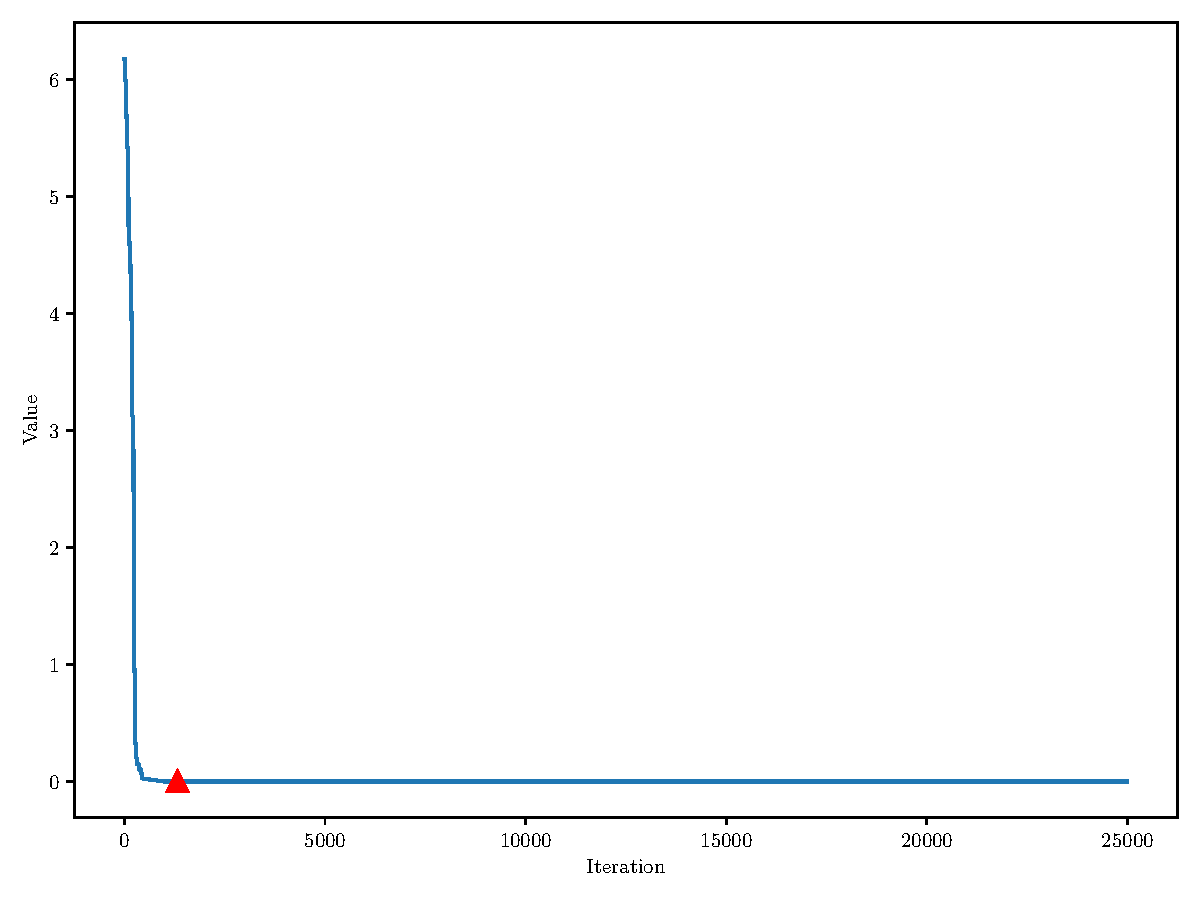
\includegraphics[width=\textwidth]{figures/Random Search_loss.pdf}
        \caption{最优值收敛曲线}
    \end{subfigure}
    \begin{subfigure}{0.4\textwidth}
        \centering
        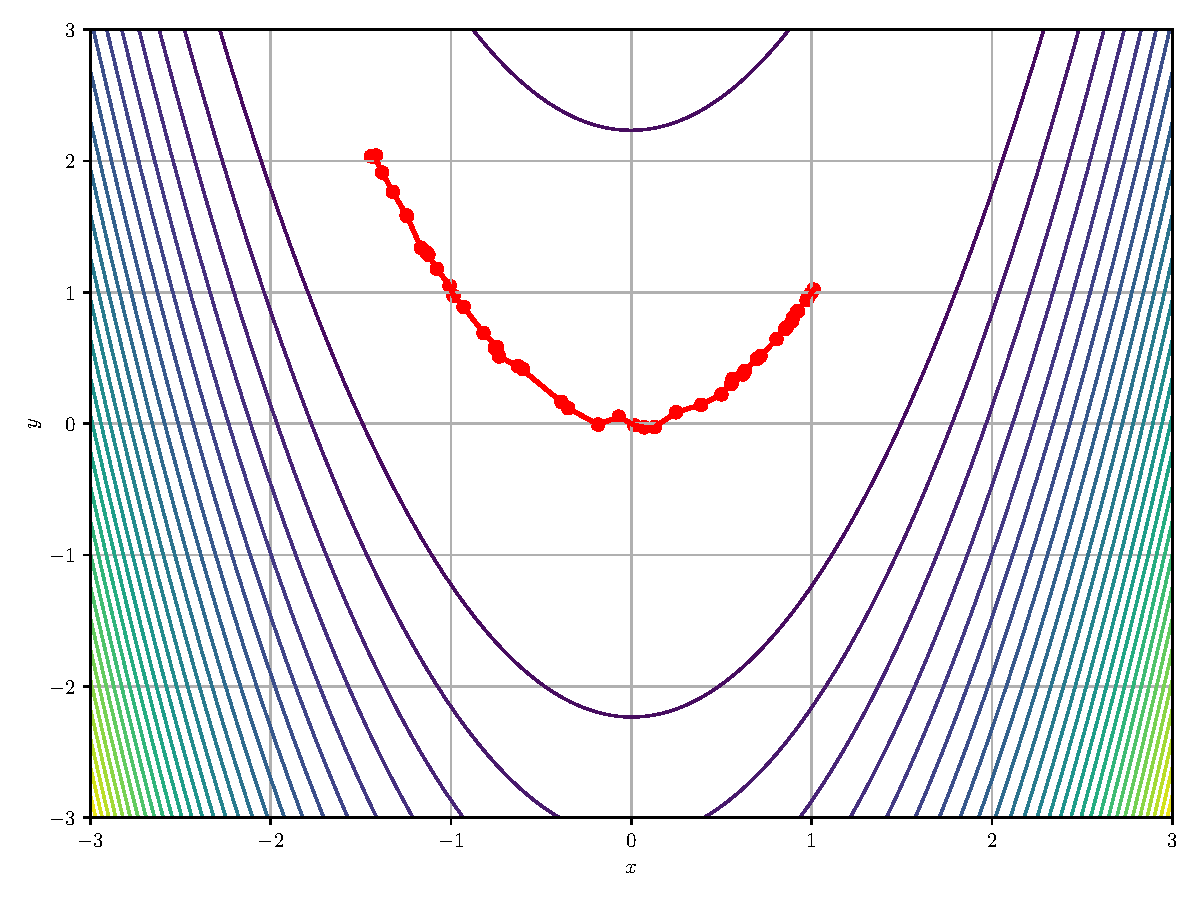
\includegraphics[width=\textwidth]{figures/Random Search_points.pdf}
        \caption{最优点收敛路径}
    \end{subfigure}
    \caption{Random Search的最优值收敛曲线与最优点收敛路径}
    \label{figure:random search}
\end{figure}
\begin{figure}[!ht]
    \centering
    \begin{subfigure}{0.4\textwidth}
        \centering
        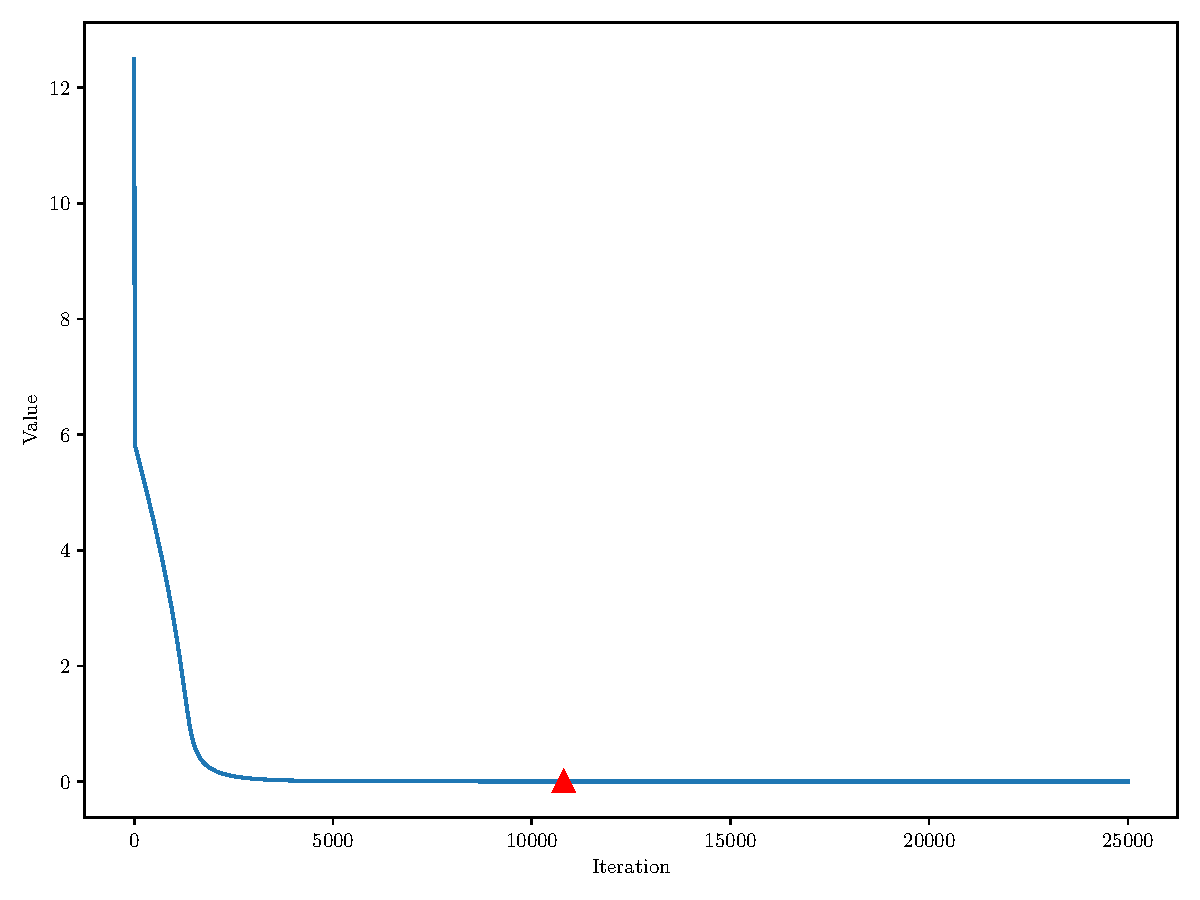
\includegraphics[width=\textwidth]{figures/Gradient Descent_loss.pdf}
        \caption{最优值收敛曲线}
    \end{subfigure}
    \begin{subfigure}{0.4\textwidth}
        \centering
        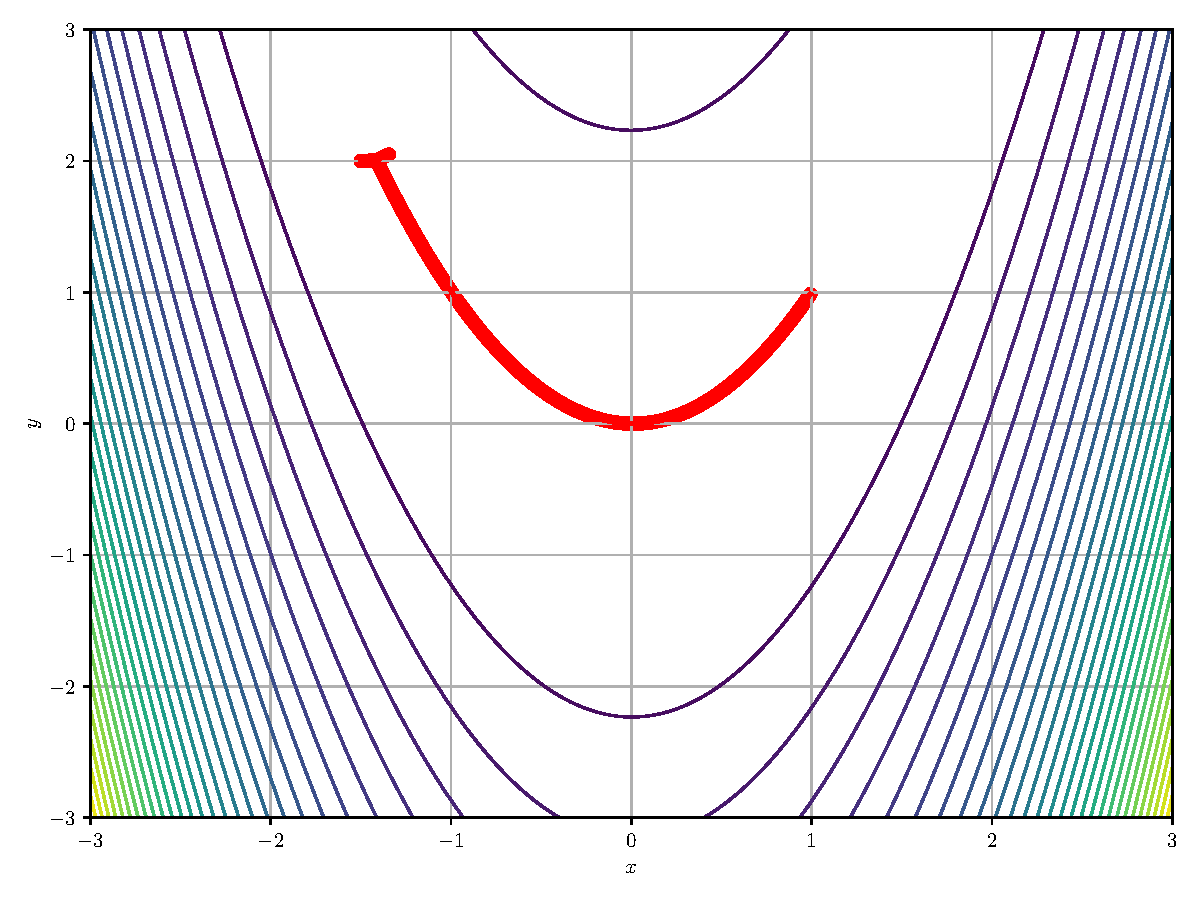
\includegraphics[width=\textwidth]{figures/Gradient Descent_points.pdf}
        \caption{最优点收敛路径}
    \end{subfigure}
    \caption{Gradient Descent的最优值收敛曲线与最优点收敛路径}
\end{figure}
\begin{figure}[!ht]
    \centering
    \begin{subfigure}{0.4\textwidth}
        \centering
        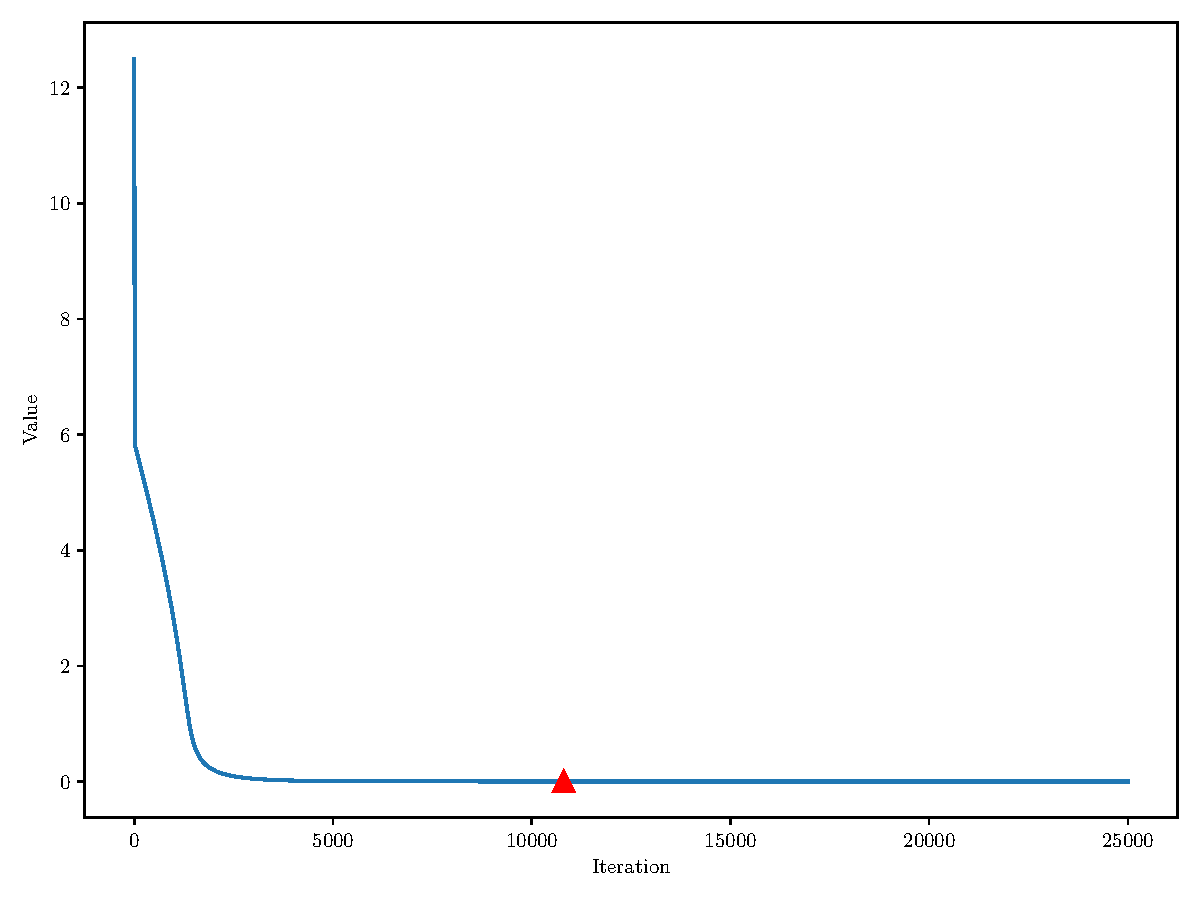
\includegraphics[width=\textwidth]{figures/Subgradient Descent_loss.pdf}
        \caption{最优值收敛曲线}
    \end{subfigure}
    \begin{subfigure}{0.4\textwidth}
        \centering
        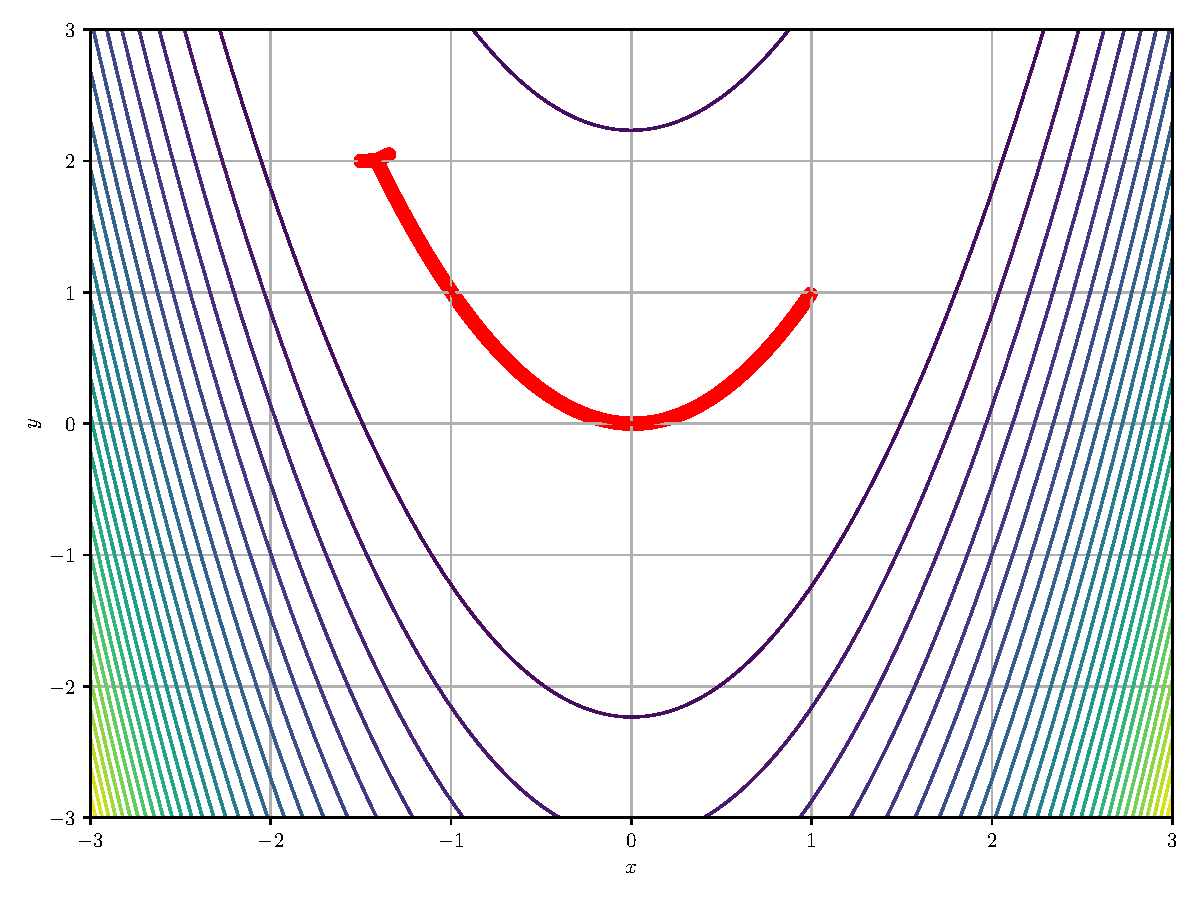
\includegraphics[width=\textwidth]{figures/Subgradient Descent_points.pdf}
        \caption{最优点收敛路径}
    \end{subfigure}
    \caption{Subgradient Descent的最优值收敛曲线与最优点收敛路径}
\end{figure}
\begin{figure}[!ht]
    \centering
    \begin{subfigure}{0.4\textwidth}
        \centering
        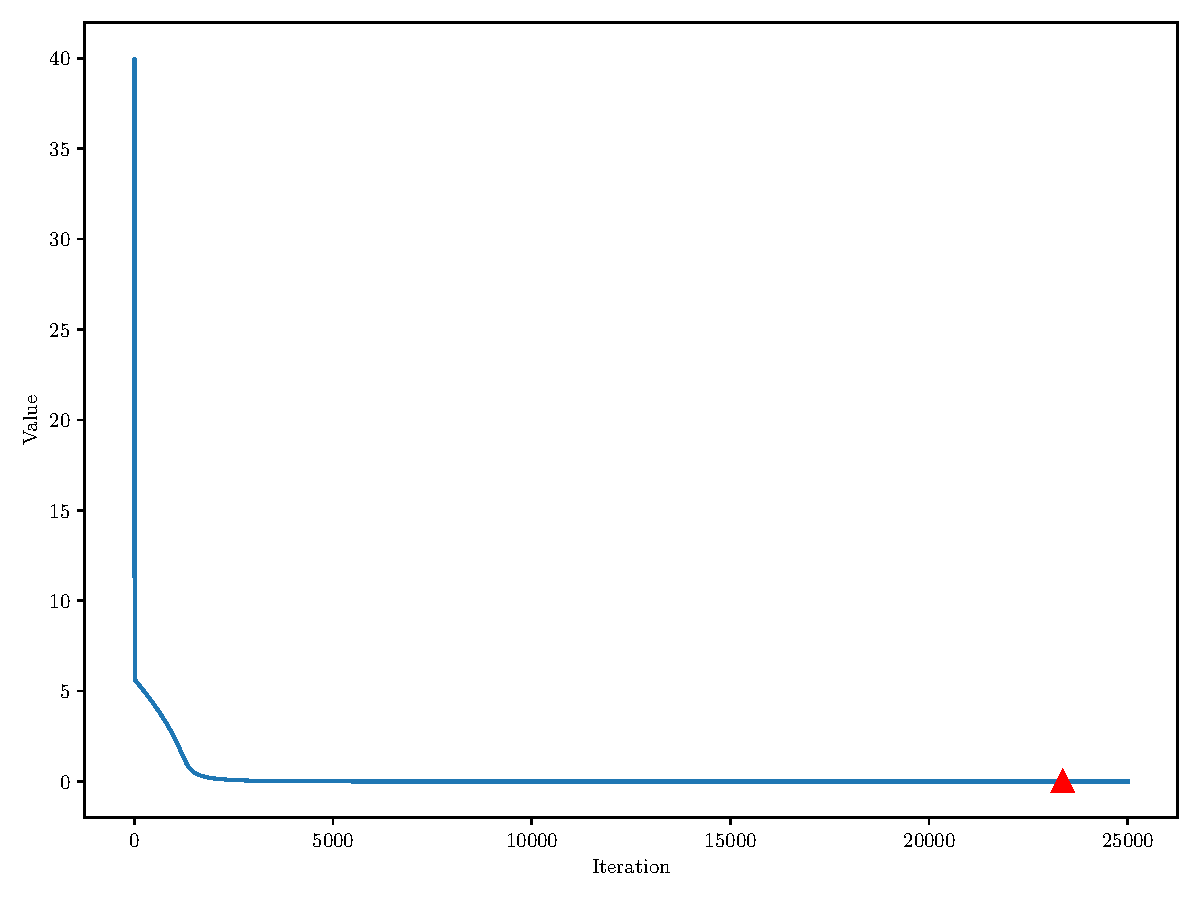
\includegraphics[width=\textwidth]{figures/Conjugate Direction_loss.pdf}
        \caption{最优值收敛曲线}
    \end{subfigure}
    \begin{subfigure}{0.4\textwidth}
        \centering
        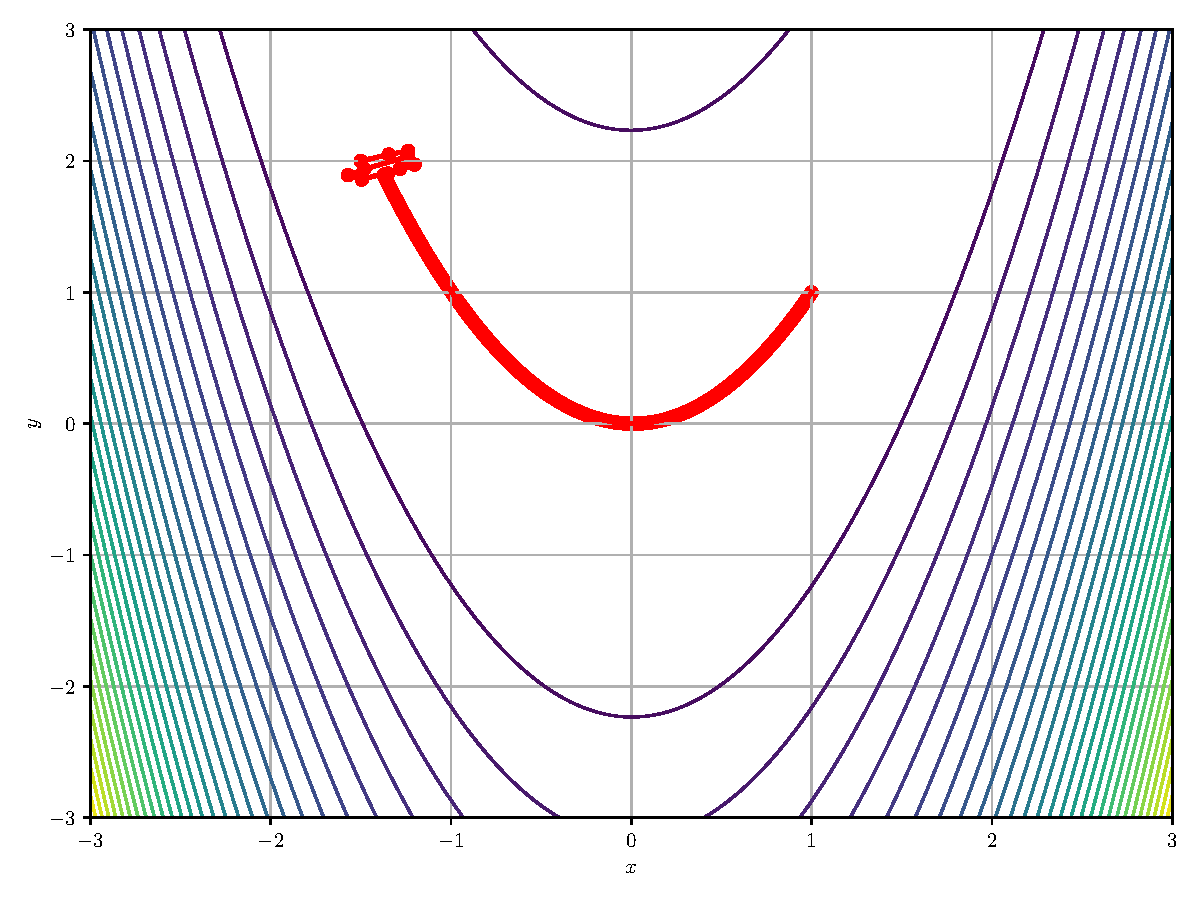
\includegraphics[width=\textwidth]{figures/Conjugate Direction_points.pdf}
        \caption{最优点收敛路径}
    \end{subfigure}
    \caption{Conjugate Direction的最优值收敛曲线与最优点收敛路径}
\end{figure}
\begin{figure}[!ht]
    \centering
    \begin{subfigure}{0.4\textwidth}
        \centering
        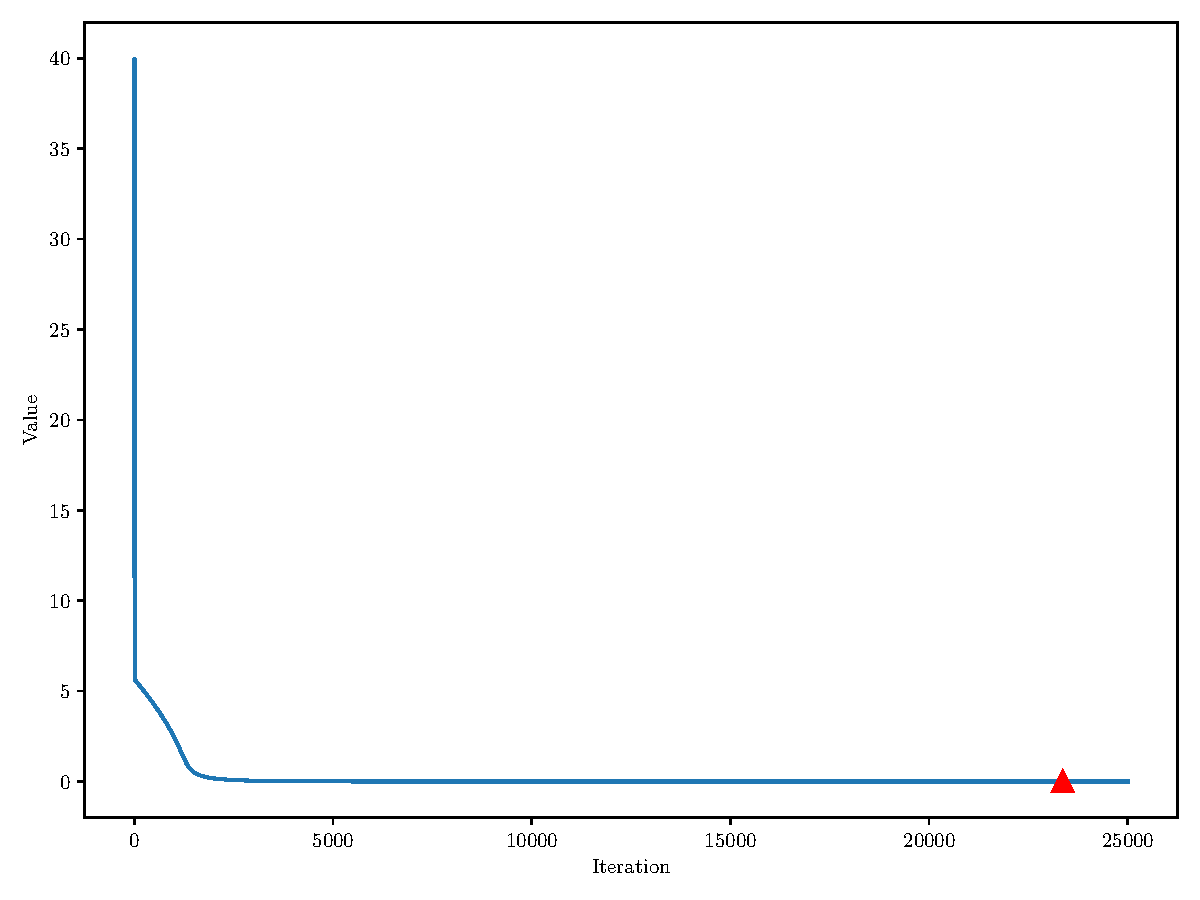
\includegraphics[width=\textwidth]{figures/Conjugate Gradient_loss.pdf}
        \caption{最优值收敛曲线}
    \end{subfigure}
    \begin{subfigure}{0.4\textwidth}
        \centering
        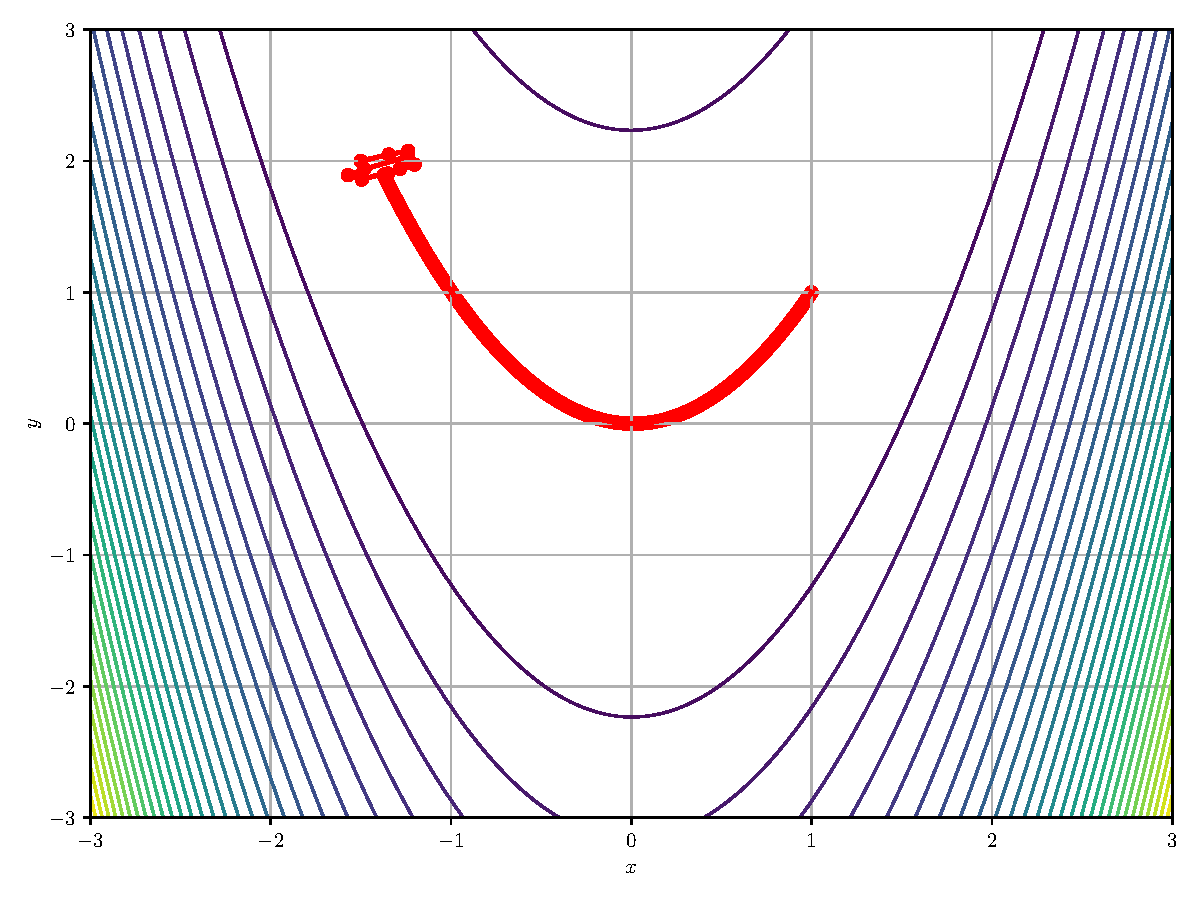
\includegraphics[width=\textwidth]{figures/Conjugate Gradient_points.pdf}
        \caption{最优点收敛路径}
    \end{subfigure}
    \caption{Conjugate Gradient的最优值收敛曲线与最优点收敛路径}
\end{figure}
\begin{figure}[!ht]
    \centering
    \begin{subfigure}{0.4\textwidth}
        \centering
        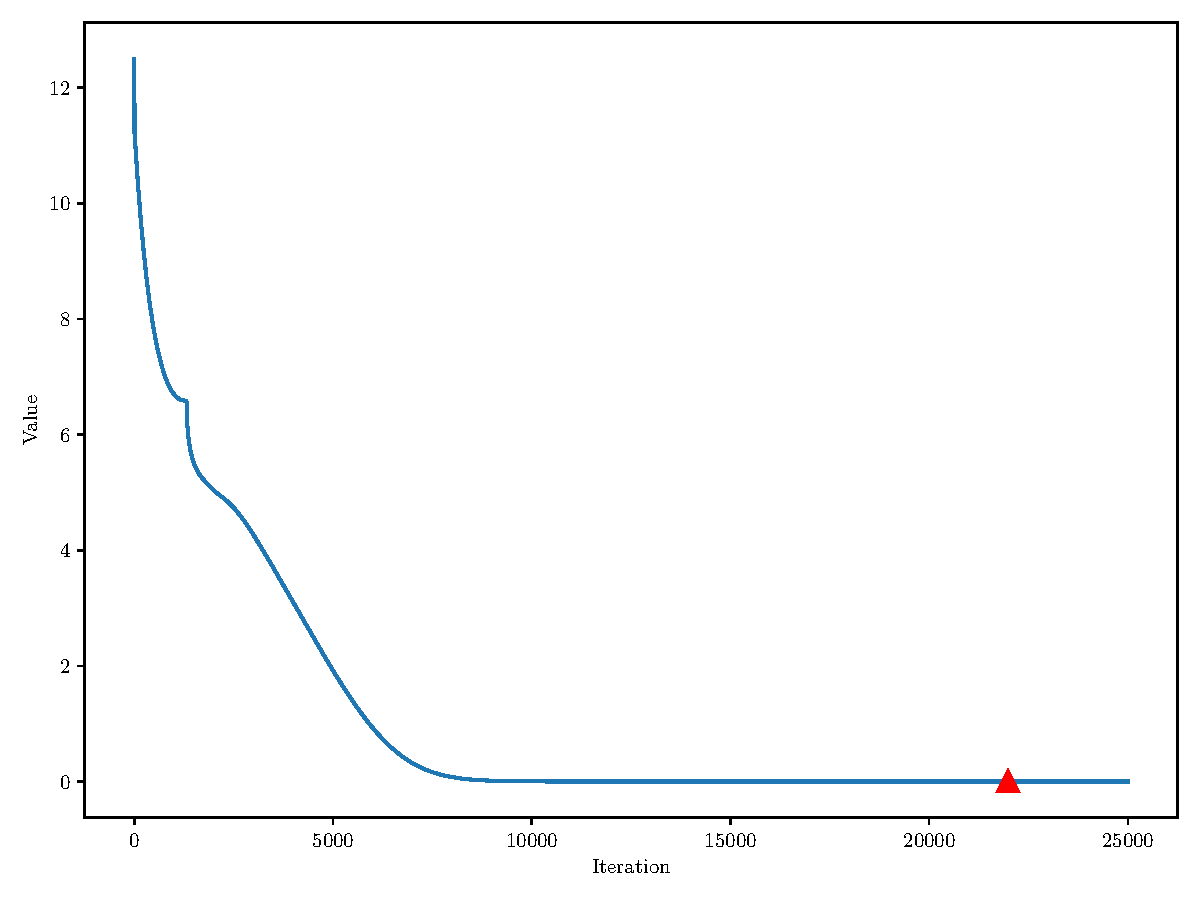
\includegraphics[width=\textwidth]{figures/BFGS_loss.pdf}
        \caption{最优值收敛曲线}
    \end{subfigure}
    \begin{subfigure}{0.4\textwidth}
        \centering
        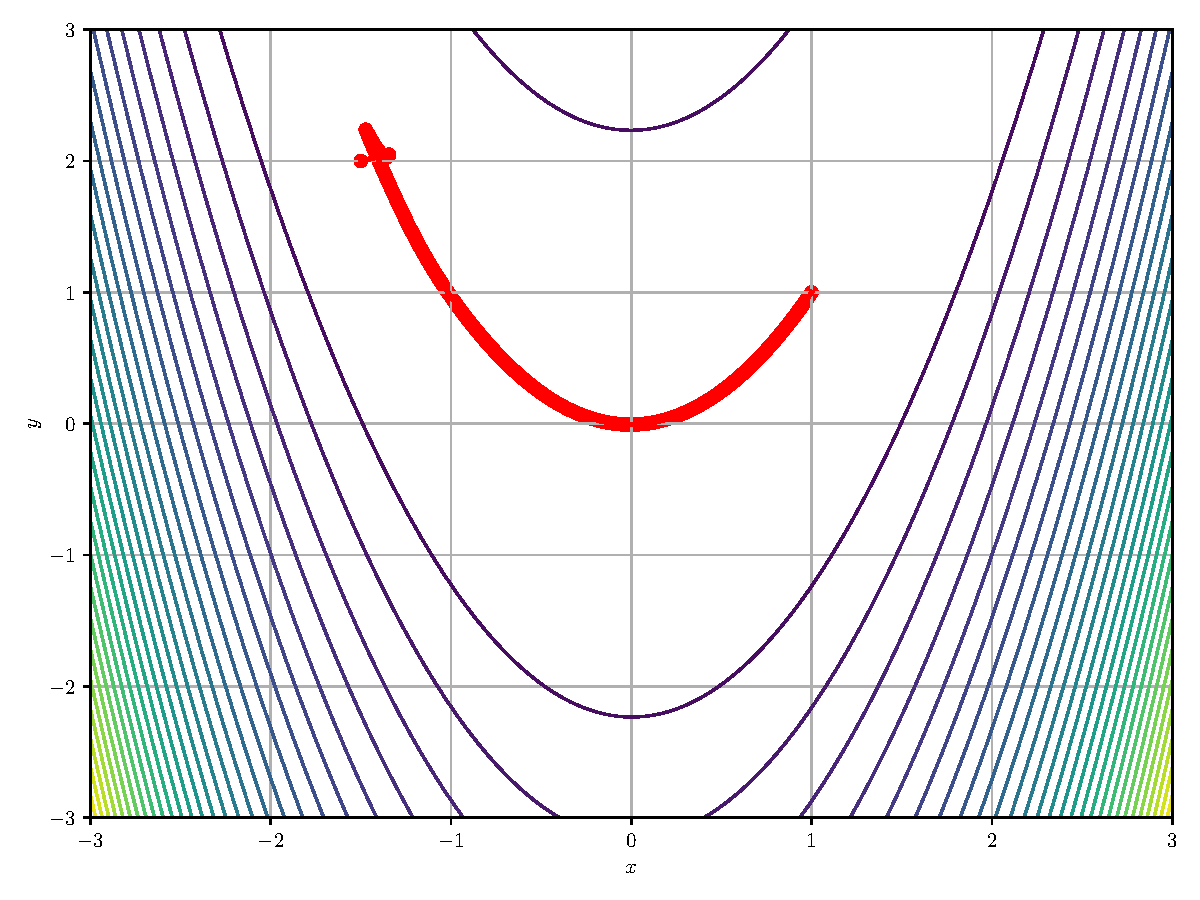
\includegraphics[width=\textwidth]{figures/BFGS_points.pdf}
        \caption{最优点收敛路径}
    \end{subfigure}
    \caption{BFGS的最优值收敛曲线与最优点收敛路径}
\end{figure}
\begin{figure}[!ht]
    \centering
    \begin{subfigure}{0.4\textwidth}
        \centering
        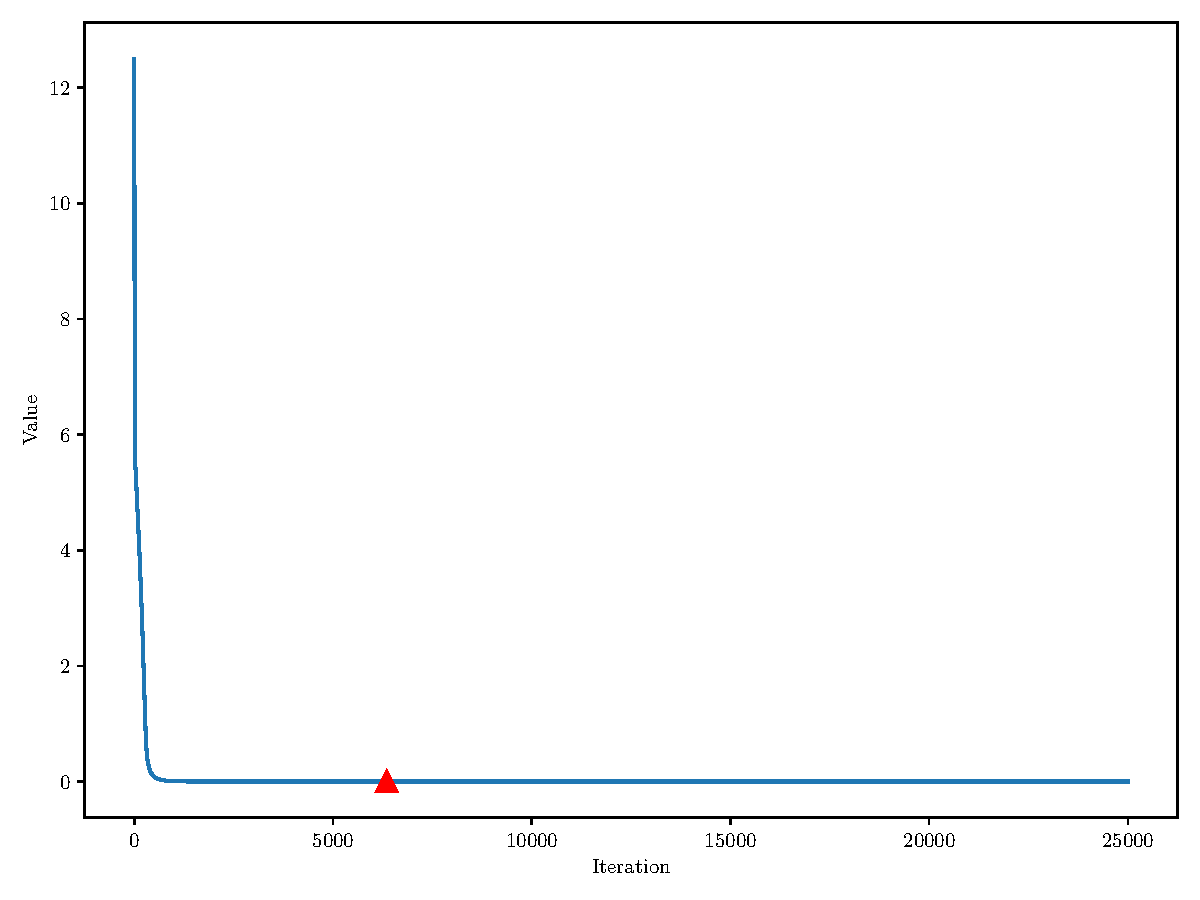
\includegraphics[width=\textwidth]{figures/SGD_loss.pdf}
        \caption{最优值收敛曲线}
    \end{subfigure}
    \begin{subfigure}{0.4\textwidth}
        \centering
        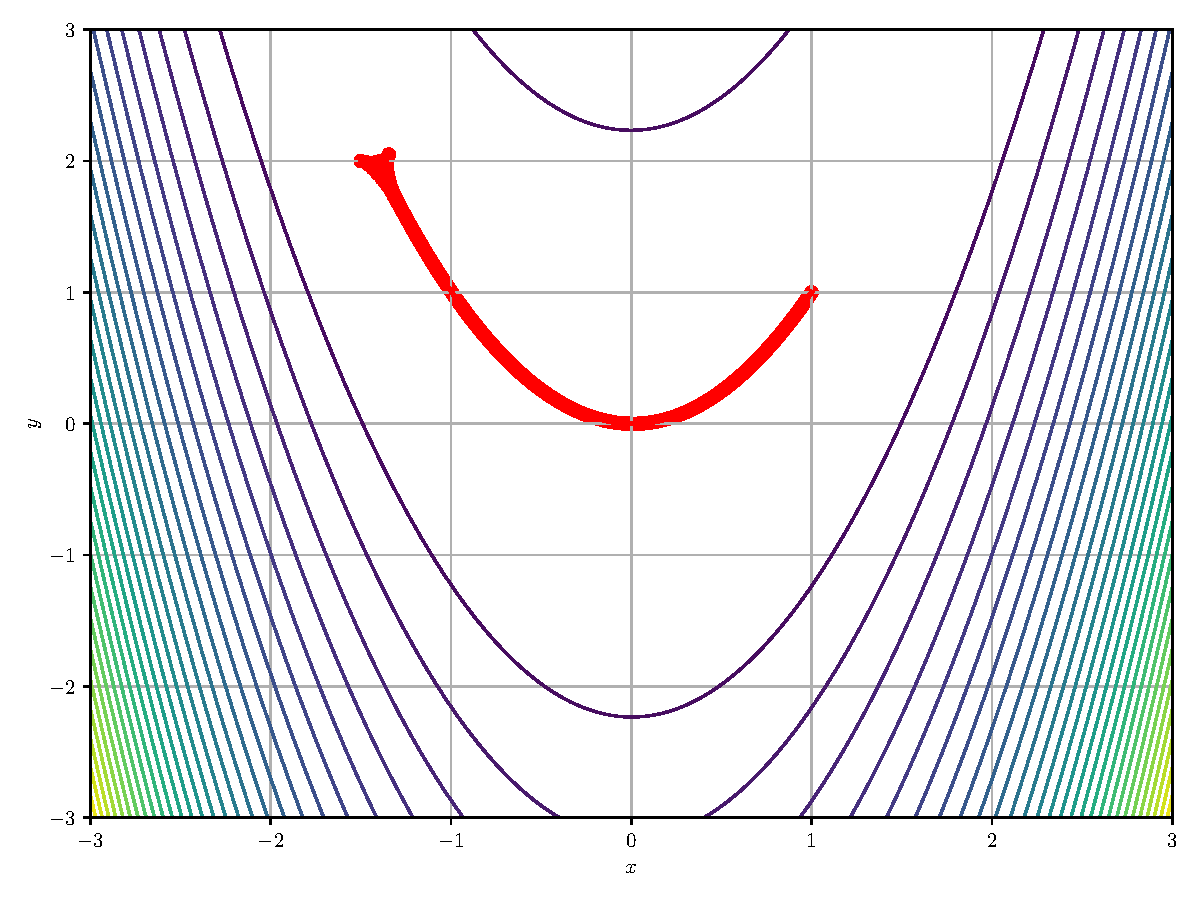
\includegraphics[width=\textwidth]{figures/SGD_points.pdf}
        \caption{最优点收敛路径}
    \end{subfigure}
    \caption{SGD的最优值收敛曲线与最优点收敛路径}
\end{figure}
\begin{figure}[!ht]
    \centering
    \begin{subfigure}{0.4\textwidth}
        \centering
        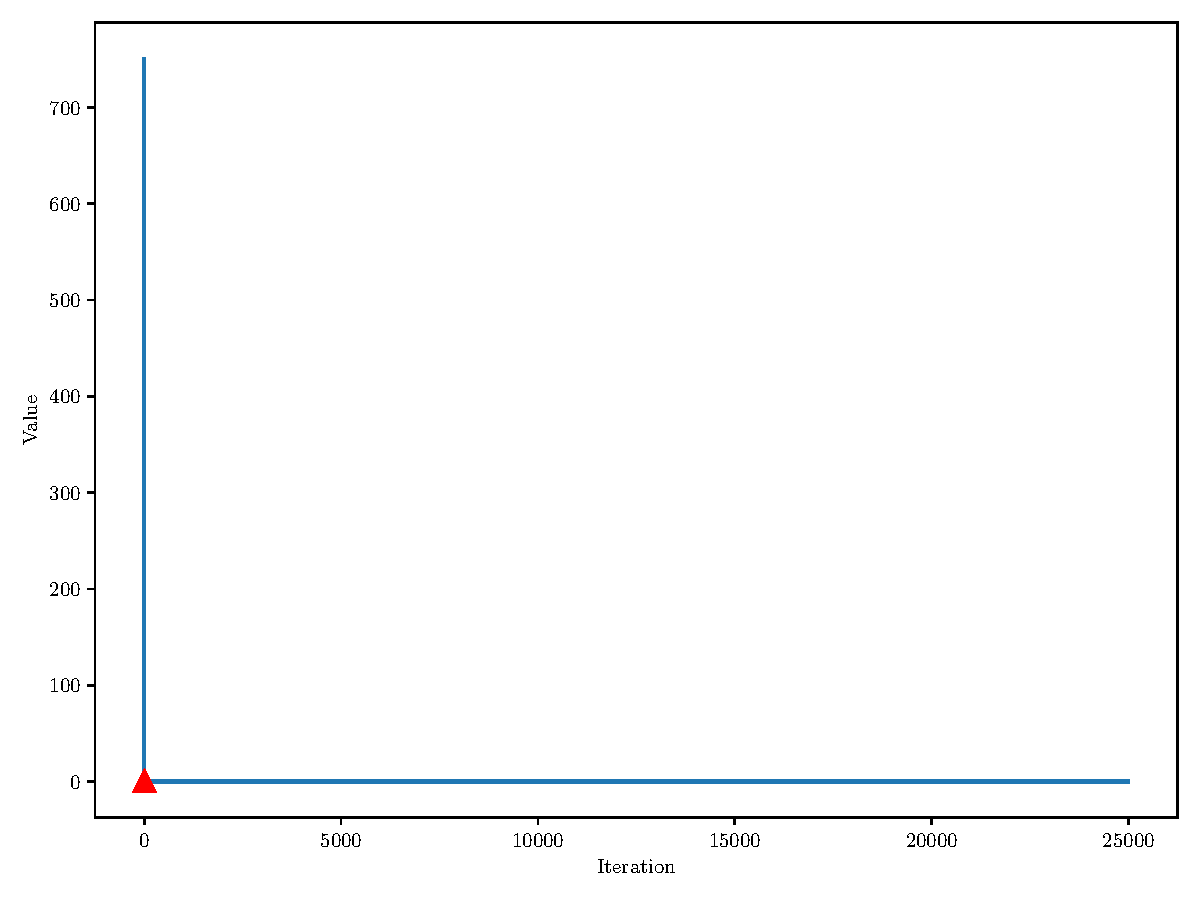
\includegraphics[width=\textwidth]{figures/Newton_loss.pdf}
        \caption{最优值收敛曲线}
    \end{subfigure}
    \begin{subfigure}{0.4\textwidth}
        \centering
        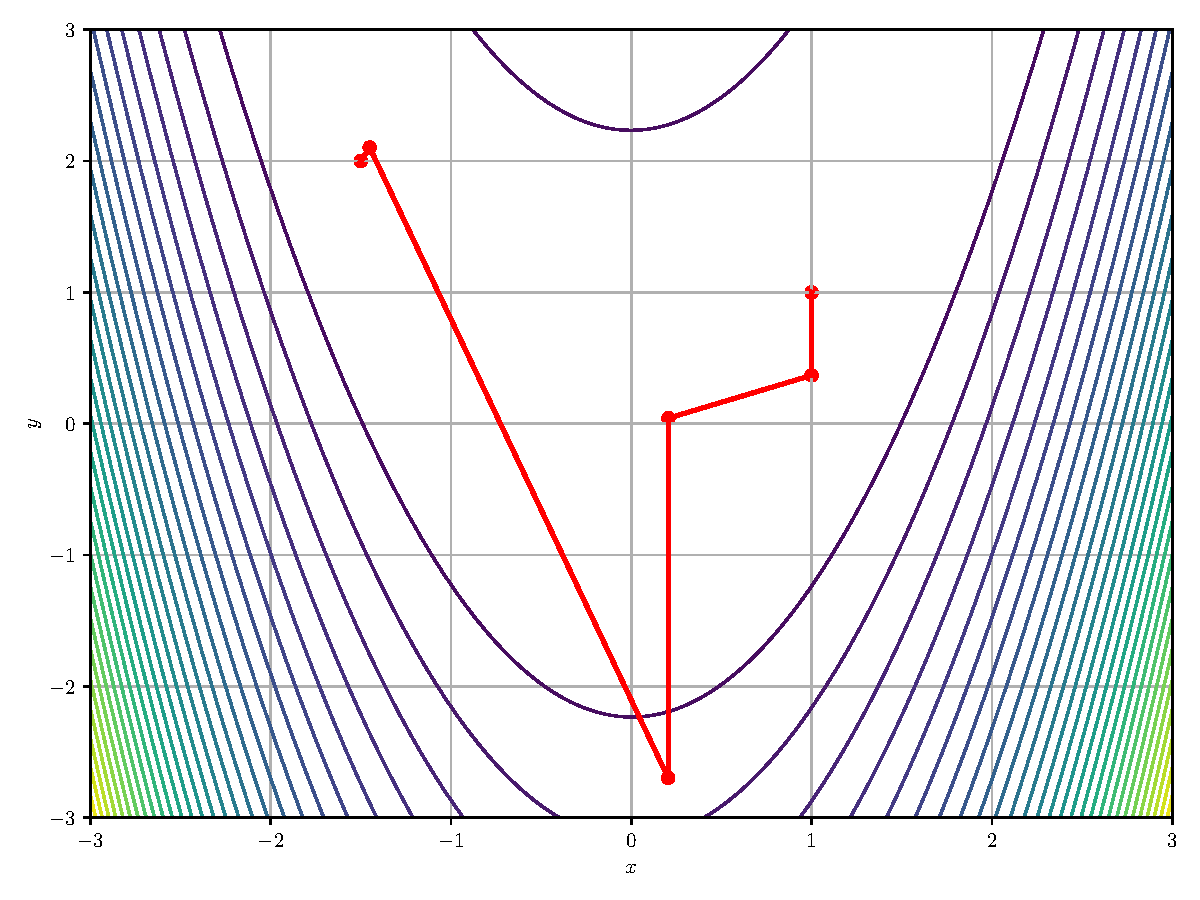
\includegraphics[width=\textwidth]{figures/Newton_points.pdf}
        \caption{最优点收敛路径}
    \end{subfigure}
    \caption{Newton的最优值收敛曲线与最优点收敛路径}
\end{figure}
\begin{figure}[!ht]
    \centering
    \begin{subfigure}{0.4\textwidth}
        \centering
        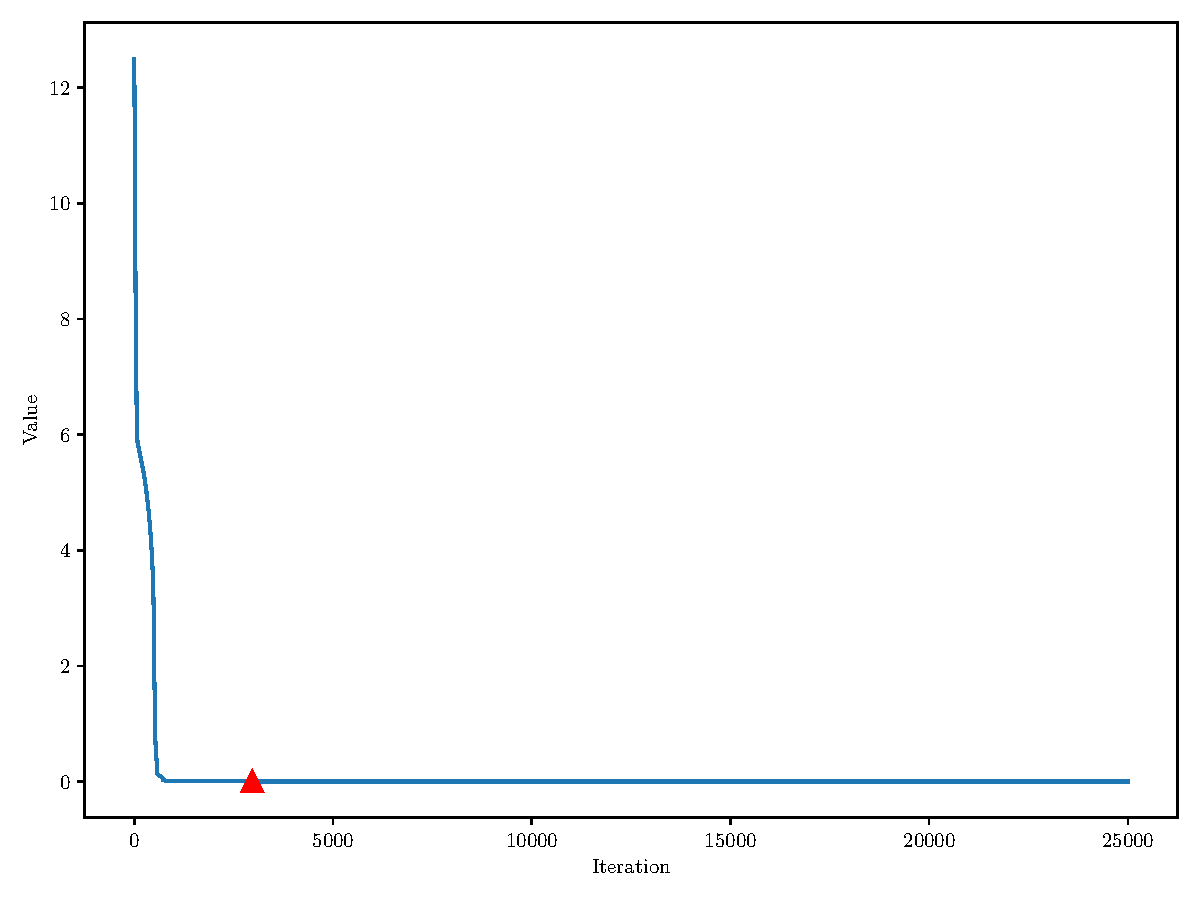
\includegraphics[width=\textwidth]{figures/Damped Newton_loss.pdf}
        \caption{最优值收敛曲线}
    \end{subfigure}
    \begin{subfigure}{0.4\textwidth}
        \centering
        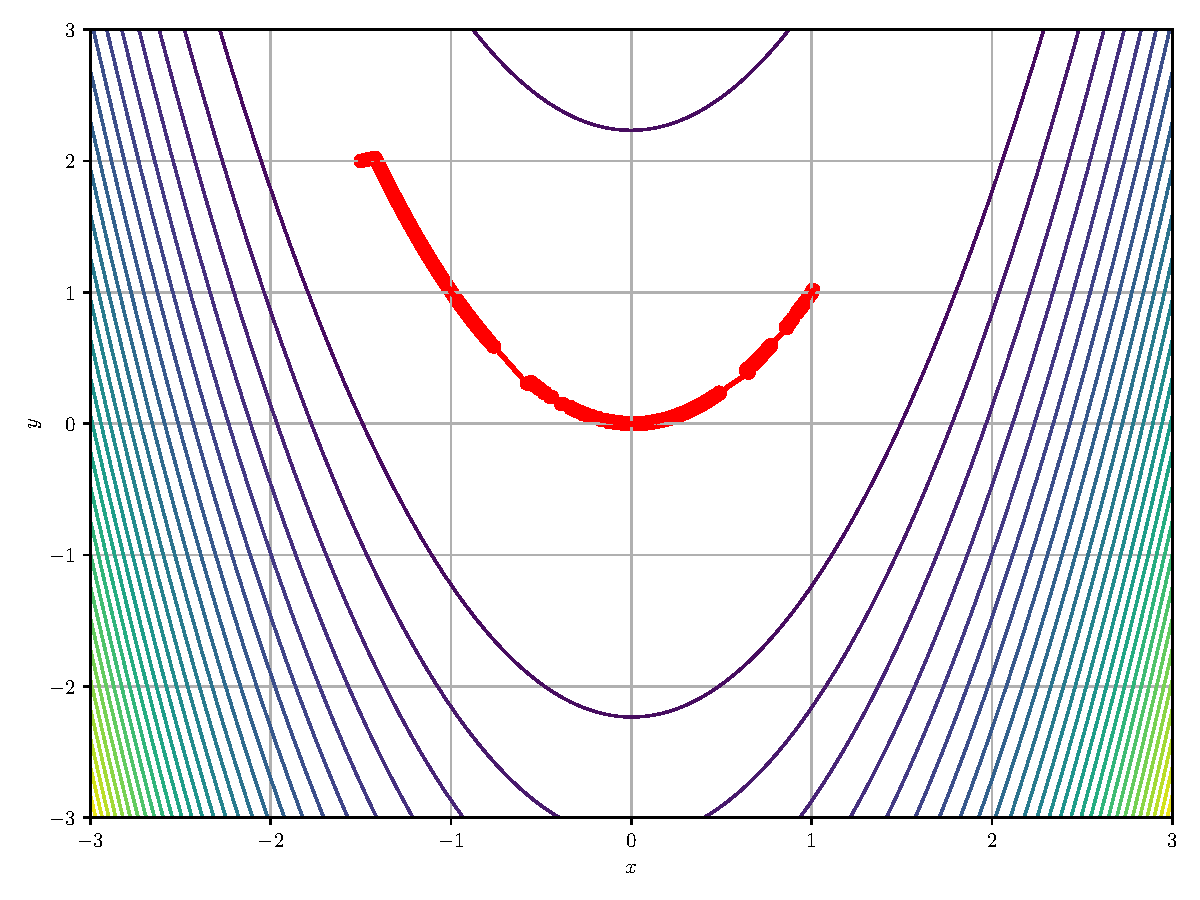
\includegraphics[width=\textwidth]{figures/Damped Newton_points.pdf}
        \caption{最优点收敛路径}
    \end{subfigure}
    \caption{Damped Newton的最优值收敛曲线与最优点收敛路径}
\end{figure}
\begin{figure}[!ht]
    \centering
    \begin{subfigure}{0.4\textwidth}
        \centering
        \includegraphics[width=\textwidth]{figures/ADMM_loss.pdf}
        \caption{最优值收敛曲线}
    \end{subfigure}
    \begin{subfigure}{0.4\textwidth}
        \centering
        \includegraphics[width=\textwidth]{figures/ADMM_points.pdf}
        \caption{最优点收敛路径}
    \end{subfigure}
    \caption{ADMM的最优值收敛曲线与最优点收敛路径}
\end{figure}
\begin{figure}[!ht]
    \centering
    \begin{subfigure}{0.4\textwidth}
        \centering
        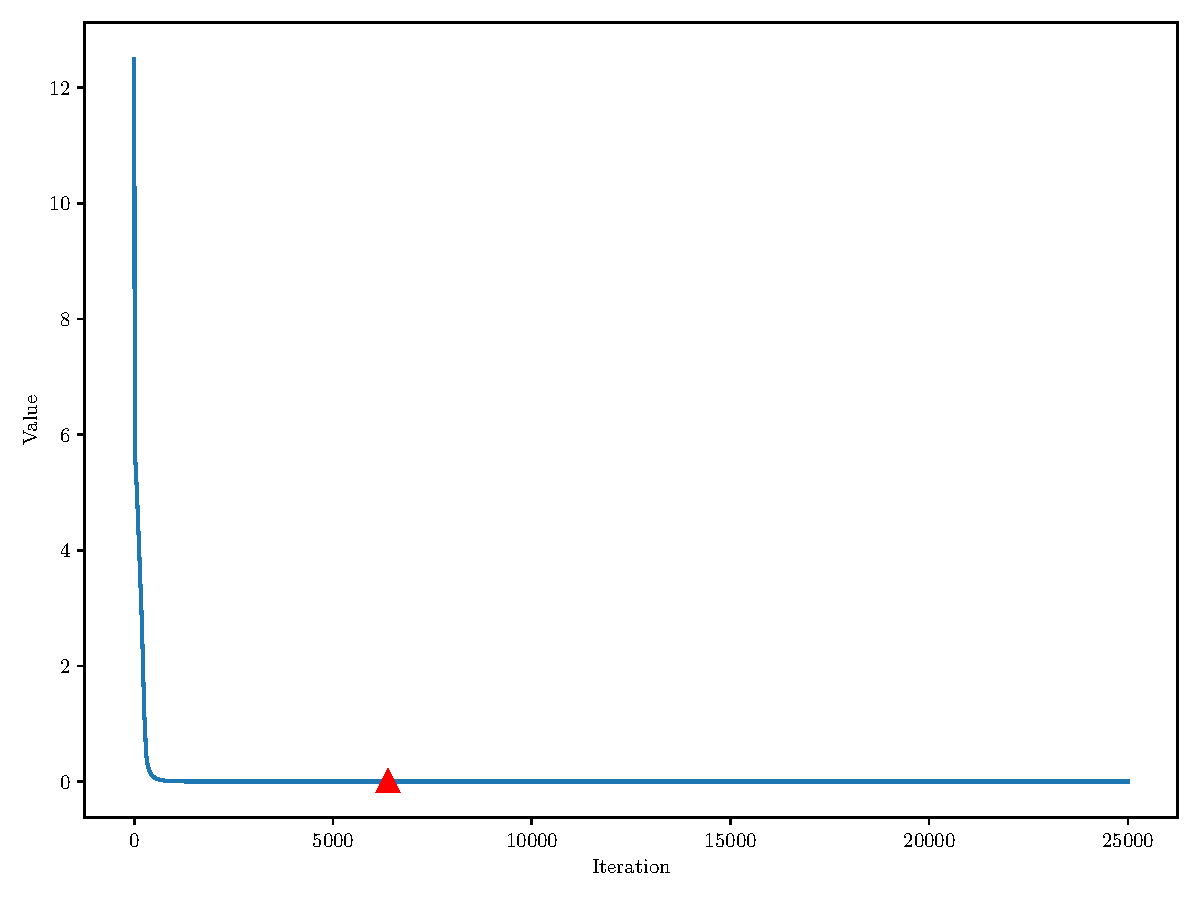
\includegraphics[width=\textwidth]{figures/Krylov_loss.pdf}
        \caption{最优值收敛曲线}
    \end{subfigure}
    \begin{subfigure}{0.4\textwidth}
        \centering
        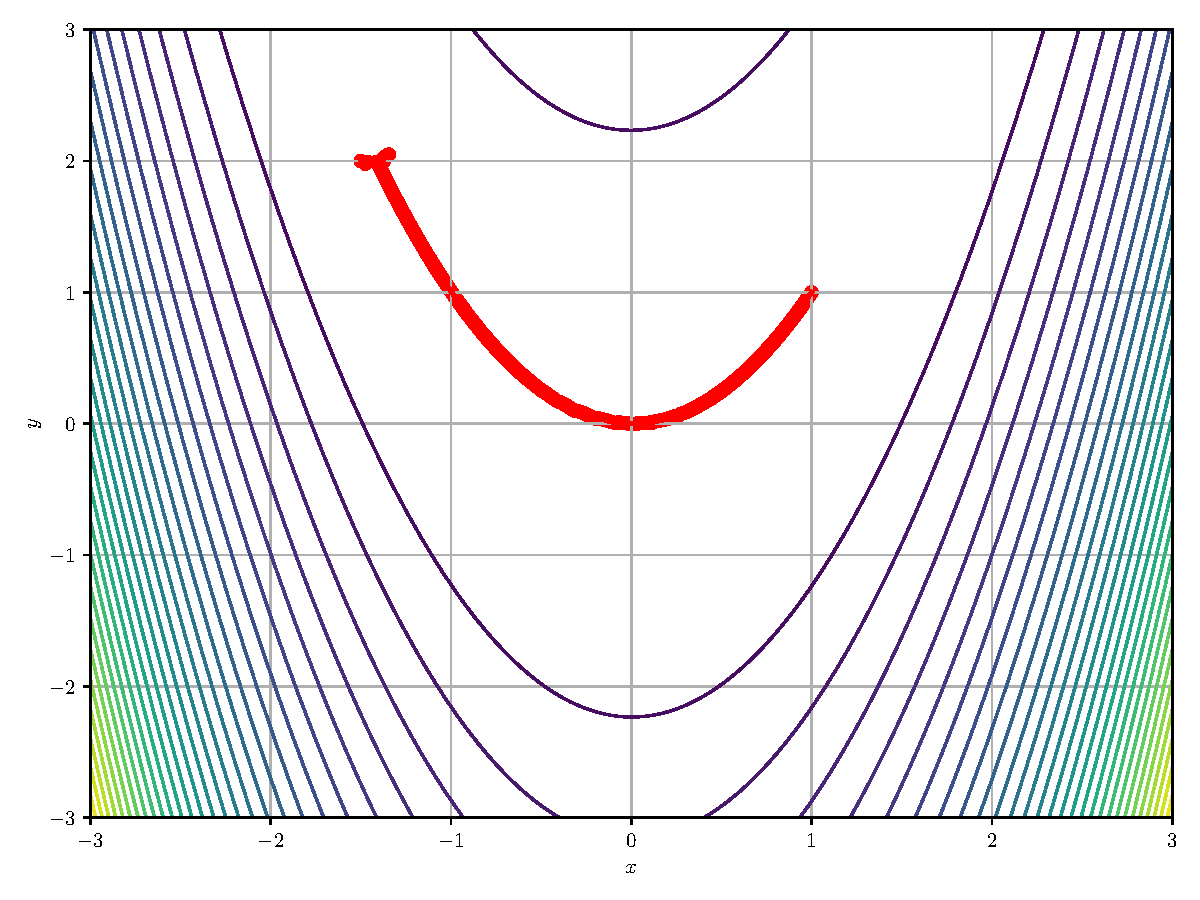
\includegraphics[width=\textwidth]{figures/Krylov_points.pdf}
        \caption{最优点收敛路径}
    \end{subfigure}
    \caption{Krylov的最优值收敛曲线与最优点收敛路径}
    \label{figure:krylov}
\end{figure}

从各图可看出,各优化器均在较少的迭代轮次内下降至最优值附近,但各优化器迭代至最优点需要的迭代轮次总和不同。
综合\cref{table:result}可知,Newton法所需要的迭代轮次最少。

鉴于Random Search优化器对初始随机种子较为敏感,实验对多个随机种子进行了实验比较,结果显示使用种子42时所需迭代轮次较少,因此在实验中固定采用该种子。

从\cref{figure:random search}中可看出,Random Search优化器也在较少的迭代轮次下收敛到最优点。
